
\chapter{Summary of publications} \label{ch:method}
This research on skin cancer classification based on deep learning is supported by six papers, the full-text versions of which are available in Part B. This chapter presents a short summary of how these papers support the thesis, as well as the author's contribution to each paper.

\begin{figure}[!h]
\centering
	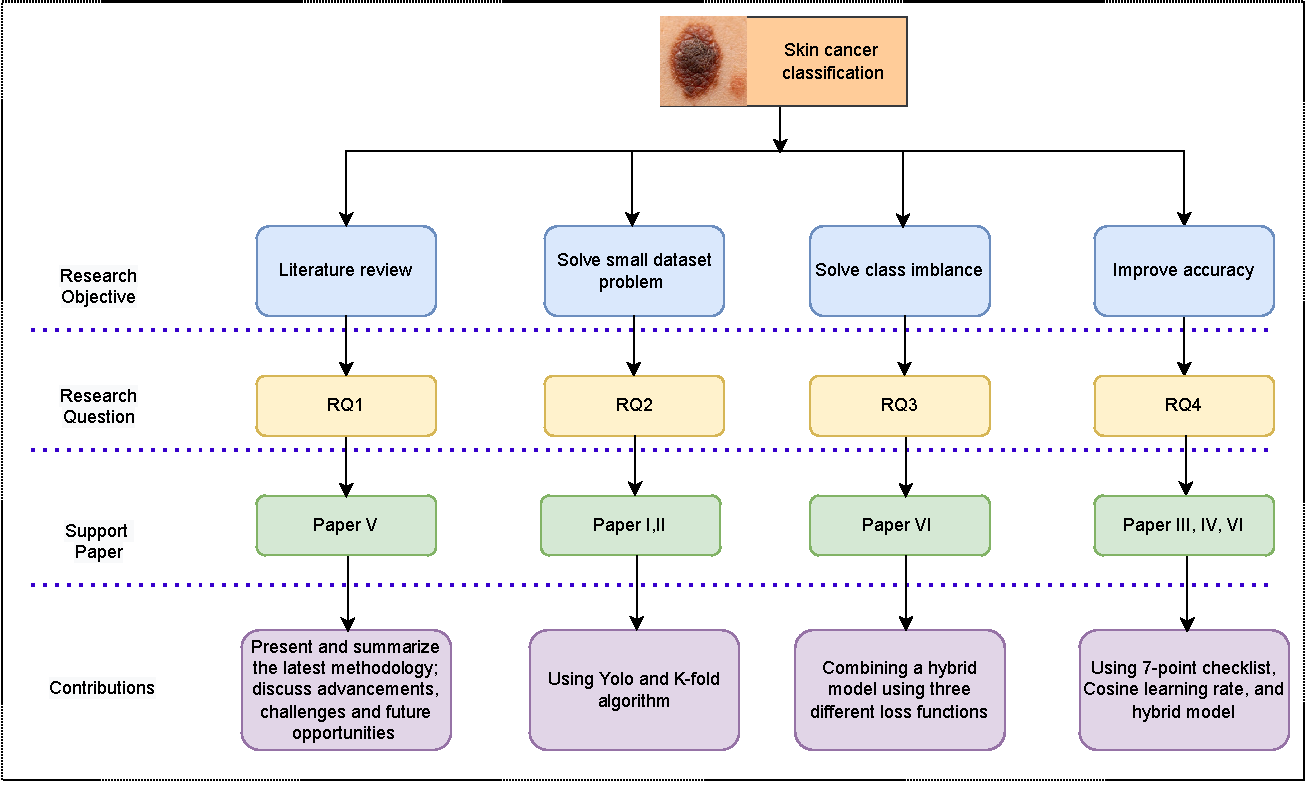
\includegraphics[width=4.2in]{map}
		\caption{Research objectives, studies, and contributions of the work.}
		\label{Fig:paper} 
\end{figure}
%map of contributions to goals of research studies

\section*{Paper I}
\textbf{Automatic Detection of Melanoma with Yolo Deep Convolutional Neural Networks}, \textit{in 2019 E-Health and Bioengineering Conference (EHB)}



~\\

Paper I addresses the small dataset problem while striving to maintain diagnostic accuracy. In Paper I, only 200 pictures were used to train the model. Yolo is a popular framework for object detection and is effective for the diagnosis of skin diseases. It not only can classify skin diseases, but also can determine the specific location of the lesion. There are three most important features of the Yolo algorithm: first, using a grid instead of a single window moving across the image; second, reducing the complex problem of classification and localization of an object to one regression problem; third, very effective generalization of knowledge. Yolo treats the detection and classification problems as a single regression problem, which puts a grid with the size of $S \times S$ on the image. For each cell of the grid, Yolo predicts whether there are objects in it and for each of them the coordinates of the rectangle surrounding the object are determined. So far, Yolo has been upgraded to eight versions, but I only used three versions at that time. The contribution of Paper I to the whole thesis is to address a small database pain point in deep learning. 

\section*{Paper II}
\textbf{Deep Melanoma classification with K-Fold Cross-Validation for Process optimization}, \textit{in 2020 IEEE International Symposium on Medical Measurements and Applications (MeMeA)}



~\\

Paper II proposes the application of a convolutional neural network-based method using K-fold cross-validation to a small skin disease database. K-fold is a validation technique in which it splits the data into $k$-subsets and the holdout method is repeated $k$-times where each of the $k$ subsets is used as a test set and other $k-1$ subsets are used for training purposes. Then the average error from all these $k$ trials is computed, which is more reliable as compared to the standard handout method. This dataset comes from the University of Salerno, which collaborated with local hospitals to collect data. The data quality is therefore high, although the data volume is relatively small. This dataset contains around 1,000 images and all annotations were made by experts. To improve the diagnostic accuracy, I used a five-fold cross-validation training dataset with Vgg-16 as the backbone to train the data. Cross-validation helps to reduce bias and therefore stabilize performance between the training dataset and the testing dataset.
 

\section*{Paper III}
\textbf{Ensembling CNNs for dermoscopic analysis of
suspicious skin lesions}, \textit{in 2021 IEEE International Symposium on Medical Measurements and Applications (MeMeA)}



~\\

Paper III focuses on improving diagnostic accuracy and using ensembling CNNs as feature extractors to diagnose suspicious skin lesions. GoogleNet, Inception-v3, and ResNet-101 were used here. The dataset used is a public dataset created according to the 7-point checklist standard and containing 1,011 images. Dermatologists usually use the weighted 7-point checklist based on pattern analysis as a diagnostic guide. Here, let the machine combine deep learning and the perspective of a dermatologist to study the skin lesion dataset. In this paper, binary classification was performed on this dataset. The classifier used the "or rule" and the majority decision. In the Datasets section of Chapter \ref{ch:theory}, I have introduced the 7-point checklist in detail. 


\section*{Paper IV}
\textbf{Skin Cancer Classification based on Cosine Cyclical Learning Rate with Deep Learning}, \textit{in 2022 IEEE International Instrumentation and Measurement Technology Conference (I2MTC)}



~\\

Paper IV also focuses on improving diagnostic accuracy. It used three different learning rates for training, while using three different backbones, i.e., Vgg-19, ResNet-101, and Inception-V3. The learning rate is one of the most important hyperparameters when it comes to training a neural network. It determines the magnitude of weight updates. It is also the trickiest parameter to set because it can significantly impact model performance. Cyclical learning rates enable learning rates to oscillate back and forth between a lower and upper bound. The benefits are that have more freedom in initial learning rate choices and break out of saddle points and local minima. The dataset used is the large Ham10000 dataset.

\section*{Paper V}
\textbf{Recent Advances in Diagnosis of Skin Lesions Using Dermoscopic Images Based on Deep Learning}, \textit{in 2022 IEEE Access}



~\\

Paper V  is mainly a literature review of the research on deep learning for skin disease diagnosis published between 2017 and 2022. This paper presents the challenges of melanoma classification based on dermoscopic images, reviews common methods and novel methods to improve accuracy, and offers guidance for future research directions. This paper present and summarize the latest methodology in melanoma classification and the techniques to improve this. It discusses advancements in deep learning-based solutions to diagnose skin cancer, along with some challenges and future opportunities to strengthen these automatic systems to support dermatologists and enhance their ability to diagnose skin cancer.

\section*{Paper VI}
\textbf{A Deep CNN Transformer Hybrid Model for Skin Lesion Classification of Dermoscopic Images using Focal Loss}, \textit{in 2022 MDPI Diagnostics}



~\\

Paper VI proposes a CNN Transformer hybrid model in an end-to-end fashion incorporating a focal-loss based loss function to classify skin lesion images. If the selected neural network is too deep, due to the limited number of training set samples used, 
this leads to overfitting of the network, but underfitting occurs if the network is chosen to be too shallow. This conclusion has been verified in many experiments. After multiple data enhancement experiments and comparisons, the LeNet network model has an accuracy of about 76$\%$ in the classification of skin cancer images, the AlexNet model an accuracy of about 79$\%$, the GoogLeNet model an accuracy of about 83$\%$, and the ResNet network model a stable accuracy of 85$\%$. Therefore, this paper chose the ResNet model because of its better image classification. Currently, the mainstream ResNet model is divided according to the depth of the network, there being four types: ResNet-50, ResNet-101, ResNet-152, and ResNet-200. Since the networks of ResNet-152 and ResNet-200 are too deep, the training is time-consuming, and when the network model layers are too deep, a large number of data is required to derive the training parameters. The size of the training set in this paper was limited, so only the ResNet-50 network model was selected for the experiment.

In general, the focal loss function is chosen as it is more appropriate for counting the contributions of samples that are difficult and easy to classify, respectively, to the total loss. The underlying idea of the focal loss function was regarded as especially suitable for the research content of this article. Through the focal loss function, the contribution of easily misclassified malignant melanoma images 
 to the total loss can be increased, and the relatively large number of benign skin diseases that are easily classified can be reduced. %The contribution of the image to the total loss.
% \begin{figure}
% \centering
% 	\includegraphics[width=2.2in]{figures/ddist2.png}
% 		\caption{Flying altitude.}
% 		\label{Fig:side} 
% \end{figure}


% % In this placement, every dome inscribes a regular hexagon, such that its sides are equal to $r$. The overlapping between each two domes has a length of $r$ and height ,$h$, of $\frac{1}{2}\times r$.

% In this placement, every three adjacent noncollinear domes form an equilateral triangle. Its side, $s$, is the distance between the centers of the two adjacent domes, Fig. \ref{fig:before}. That distance equals to $2 \sqrt{(r^2)- (h^2)}$.
% and its altitude, $t$, equals to $\frac{\sqrt{3}}{2} \times s$.
% This placement provides full coverage on the ground level. In 3D volume, intersection points of every three adjacent noncollinear domes would be blind spots with zero coverage at the flying altitude as shown in Fig. \ref{fig:before}. Therefore, domes should be re-positioned in order to provide full coverage at the defined altitude. 


% In order to cover the blind spots while keeping the thinnest hexagonal pattern, the altitude $t$ should be reduced by $d$ in Fig. \ref{Fig:side}. Therefore, the new triangle side $s'$, which represents the distance between domes center, is equal to: 

% \begin{equation} \label{eq:dist}
%   s' = s - 2d /\sqrt{3}
% \end{equation}
% Re-positioning the domes provides full coverage of the volume, including intersection points as shown in Fig. \ref{fig:after}. It also changes the minimum overlapping height, $h$, between adjacent domes that ensure 100\% detection at flying altitude $a$. This height can be calculated as the apothem of the equilateral triangle, which equals to:

% \begin{equation} \label{eq:height}
%     h = t/3
% \end{equation}

% \begin{figure*}[h]
  
%     \subfloat[Thinnest covering with blind spots ]{{\includegraphics[width=0.49\linewidth,height=2in]{figures/place-before2.png}
%     \label{fig:before}}}
%     %\hspace{0.5em}
%     \subfloat[Full coverage placement]{{\includegraphics[width=0.49\linewidth,height=2in] {figures/place-after3.png}
%     \label{fig:after}}}
 
%     \caption{Hexagonal placement of camera domes.}
%     \label{fig:place2}
% \end{figure*}
% The flying altitude is used as a constraints to re-position while guaranteeing 100\% detection. In Fig. \ref{Fig:place2}, 


% Two placement constraints defined are, the dome capacity and the maximum flying altitude $a$. The dome capacity is obtained from its coverage radius $r$ multiplied by the minimum pixel resolution required for detection at that distance. For example, if the coverage radius of the dome is 500 meters and the required minimum detection resolution is 10 pixels at 500 meters, then the dome capacity is 5000.
% %pixels per meter (pix/m).
% The flying altitude $a$, should not be more that $r$, in order to ensure that the object is detected all the time it is flying within the covered volume. 
% We used the flying altitude as a constraints to calculate how much to move the nodes to cover the blind spots



% \begin{figure}
% \centering
% 	\includegraphics[width=0.5\linewidth,height=3in] {figures/placement.pdf}
% 		\caption{Coverage blind spot in hexagonal placement}
% 		\label{Fig:blind} 
% \end{figure}

% \begin{figure}
% \centering
% 	\includegraphics[width=\linewidth]{figures/placement1.png}
% 		\caption{Blind coverage spot when the direct application of hexagonal placement}
% 		\label{Fig:place1} 
% \end{figure}


% \subsection{Placement Evaluation}

% The optimized placement method discussed in \ref{sec:hexa} should achieve 100\% detection for any object flying withing the defined flying altitude. Overlapping coverage between camera domes allows extracting object
% stereoscopic information such as size and position. These criteria should be measured in order to assess the multi-camera placement.

% The method developed in \cite{paper1} evaluates coverage effectiveness of each dome placement in volumetric surveillance. Three monitoring objectives are defined and measured using GPS trajectories of six birds over an area of 9 $km^2$. The tracks are obtained from the work in \cite{birdstracks}. The defined criteria are detection, and positioning
% percentage of flying object; as well as the maximum pixel
% resolution captured to detect it.

% The required minimum detection resolution and the dome coverage radius define the dome capacity, Eq. \ref{eq:capacity}. Each tack composes of number of samples representing the coordinates in longitude and latitude. The altitude is assumed to be 200 meters for all tracks. These coordinates are converted to a Euclidean distance vector corresponding to each track. The dome capacity is then used to calculate the pixel resolution of each sample in the distance vector. 

% \textit{Detection percentage}, is calculated for each tack when its pixel
% resolution is higher than the required detection resolution. The defined resolution is 3 pixels per meters ($pix/m$). Whenever this resolution is fulfilled for the object flying over any of the domes, it means the object is detected. The placement method in \ref{sec:hexa} ensures 100\% detection for the six used trajectories over the defined 9 $km^2$ volume. Also, when the object detected in two domes, its position can be extracted. The \textit{positioning percentage} measures that when the birds fly withing overlapping areas. Moreover, the pixel resolution to detect the object changes as it flies closer or further the dome center. The \textit{maximum pixel resolution} gives an indication of that. 


% \section{Node Configuration}
% The aspect of optimizing surveillance system includes at its core the node optimization. To achieve that, two factors are considered; cost of the multi camera dome, \cite{paper3}, and its design, \cite{paper4}. 

% \subsection{Node Design Exploration}

%  The multi-camera dome is assumed to consist of multiple layers vertically and each layer consists of number of cameras at the horizontal level as in Fig. \ref{Fig:dome3d}. The design exploration in \cite{paper3} construct a cost efficient camera dome, subject to monitoring constraints, from a set of camera sensors and lenses combination. The combined horizontal angles of the cameras
% in one layer should cover a minimum of 360$^\circ$. The vertical
% angles of all the layers combined should cover a minimum of
% 90$^\circ$ to ensure monitoring a 2$\pi$ radian view. Cameras in one layer are identical, however it is not necessary that all layers have similar cameras. 

% %Therefore, we can assume that the dome is more than one layer, as shown in Fig. \ref{Fig:dome3d}. 

% \begin{figure}
% \centering
% 	\includegraphics[width=0.7\textwidth, height=2.1in]{figures/dome3d.pdf}
% 		\caption{Multi-camera dome architecture.}
% 		\label{Fig:dome3d} 
% \end{figure}

% For the design exploration, a number of constraints are defined. They include, the dome coverage radius, $r$, the minimum pixel resolution at distance $r$, and number of layers in the node. The method searches through available
% sensors and lenses to combine them such that the diameter of the covering lens must be equal or larger than the sensor size. Then, an exhaustive search algorithm is performed using the short-listed combinations. Each sensor-lens pair should fulfill pixel resolution constraint at the specified dome radius. The solution with the minimum cost is chosen as optimal. The search for optimal solution can be constrained for example by cost, number of cameras, or other parameters. The optimal solution has the following properties, the angle covered by all the layers vertically, total number of cameras in the node, number of cameras in each layer, and the solution cost. 

% % This method also investigates trade-offs among design parameters and constraints
% % to achieve the optimal solutions.
% The method estimates the cost of each member, $S_{ijn}$, of the solution space, $S$, subject to the defined design constraints. The objective function for the design exploration can be defined as minimizing the following cost function: 

% \begin{equation}\label{eq:costf}  
% \begin{aligned}
% & \underset{ \tilde{C}_{ijn}}{\text{minimize}}
% & & f( S ) \\ %\mathrm{f}
% & \text{subject to}
% & & d^c_i \leq d^o_j, \\ 
% &&& M_{ijn} \leq M, \\
% &&&  N \leq L, \\
% & & & \delta_{rijn}  \geq \delta, \\
% & & & A_{ijn} \geq \frac{\pi}{2} + \varepsilon \cdot (N-1) 
% \end{aligned}
% \end{equation}
% where $d^c_i$ and $d^o_j$ is the diameter of sensor and the covering lens, respectively, $M_{ijn}$ is the number of cameras required by the solution, 
% $A_{ij}$ is the total vertical angle covered by all layers, $N$, and $\delta_{rijn}$ is the pixel resolution in the optical plane of the FoV for the combination of camera $i$ and lens $j$ at distance $r$ from the dome for each layer $n$ in the solution.

% \subsection{Node Cost Optimization} \label{sec:cost}
% The optimized placement method in \ref{sec:hexa} motivates the inclusion of the placement in the node design. In the hexagonal placement, domes overlap in order to achieve full coverage. Also, volumes above the monitoring height are not required to be monitored. This results in coverage overhead as shown in Fig. \ref{Fig:overa}. Moreover, the coverage of each dome without the overlap in the hexagonal pattern can be modeled as a hexagon, Fig. \ref{Fig:overb}.

% \begin{figure*}
% \centering
% \subfloat[Side view]{\includegraphics[width=2.7in, height=1.3in]{figures/fig3b.png}%
% \label{Fig:overa}}
% \hfil
% \subfloat[Top view]{\includegraphics[width=1.5in]{figures/fig3a.png}%
% \label{Fig:overb}}
% \caption{Coverage of multi-camera domes in hexagonal placement.}
% \label{Fig:overhead}
% \end{figure*}
% % \begin{figure}
% % \centering
% % \includegraphics[width=3in, height=1.3in]{figures/fig3b.png}%
% % \caption{Coverage overhead in hexagonal placement.}
% % \label{Fig:overhead}
% % \end{figure}

% Taking these points into account leads to changes in node design in order to avoid coverage overhead in the hexagonal placement. Therefore, in \cite{paper4} the hemispherical design of the node is optimized accordingly. The monitored volume for each dome is
% modeled as a cylinder instead of a hemisphere, Fig. \ref{Fig:cylinder:b}. Non-overlapping volumes have a minimum
% coverage radius equals to the monitoring height. Overlapping volumes coverage radius is be bounded by the cylinder radius, $r_c$. The resulting cylindrical dome is then divided into layers, and each of them has its coverage radius. Monitoring requirements should be met at that distance. At the top layer, cameras are stacked with multiple overlap at the horizontal level. This also causes coverage overhead. Therefore, only one camera can be mounted at the top layer, Fig. \ref{Fig:cylinder:a}. That layer can be considered as a half layer when arranging the layers vertically from bottom up to cover a minimum of 90$^\circ$.
% The minimum coverage radius of each layer is defined based on the monitoring height, $h$. 

% \begin{equation}
%   {{r}_{L}}=\begin{cases}
%     {{r}_{c}}/\cos (c_A), & \text{if $x\And y<h$}.\\
%     {{r}_{m}}, & \text{if $x>h\And y<h$}. \\
%     h/\sin (p_A), & \text{if $x\And y>h$}.
%   \end{cases}
%     \label{eq:9}
% \end{equation}
% where x and y are height of the current and previous layer respectively, as shown in Fig. \ref{Fig:cylinder:b} for layer 2. ${c_A}$ is the covered vertical angle of the current and previous layers. ${p_A}$ is the vertical angle of view of the previous layer. The vertical angle of view for each layer is calculated as:

% \begin{equation}
%  v_A=2\arctan ({{d}_{v}}/2f)
%   \label{eq:11}
% \end{equation}
% where ${{d}_{v}}$ is the sensor's vertical dimension and $f$ is the lens focal length. Each layer's height is calculated as:
% \begin{equation}
%   {h}_{L}=|{{r}_{m}}.\sin ({c_A)}| 
%       \label{eq:10}
% \end{equation}

% \begin{figure*}
% \centering
% \subfloat[]{\includegraphics[width=1.0in]{figures/fig5a.png}%
% \label{Fig:cylinder:a}}
% \hfil
% \subfloat[]{\includegraphics[width=2.8in]{figures/fig5b.png}%
% \label{Fig:cylinder:b}}
% \caption[Optimized cylindrical dome design]{(a) Camera's field of view in 3D, (b) Optimized cylindrical dome design with one camera on the top layer. }
% \label{Fig:cylinder}
% \end{figure*}

% \section{Object Detection and Positioning}
% For the problem of sky monitoring in wind farms, object detection is an essential surveillance task. To investigate methods for in-flight birds detection, the performance of state of the are deep learning YOLOv4, \cite{yolov4}, is compared to computer vision based detection using background subtraction. An improved YOLO-based model is developed in \cite{paper6} and it achieves detection accuracy on testing sets of 90\% and 92\% using the datasets in \hl{dataset}\cite{mydataset}.

% %\subsection{Background subtraction}
% \subsection{Deep Learning based Object Detection}
% \subsubsection{Dataset Acquisition:}
% Object detection using deep learning requires annotated datasets for
% training, validation, and~testing. There were not any available datasets for in-flight bird that can be used in this study. Therefore, datasets were collected by Mid Sweden university in two wind farms in Denmark over the
% course of a few months in 2017 and 2018. The datasets were manually annotated using the open source annotation tool \textit{LabelImg}, \cite{labelimg}.

% \begin{figure}
%  \includegraphics[width=0.99\linewidth]{figures/dataset.pdf} 
% \caption[Example frames from Skagen and Klim datasets]{Frames from Skagen dataset (left), Klim dataset (middle), and examples of birds from both datasets with the corresponding pixels count for each box (right).}
% \label{Fig:datasets}
% \end{figure}

% \begin{figure}
% \centering
% \subfloat[]{\includegraphics[width=0.45\linewidth,height=1.5in]{figures/skagen-hist.png}%
% \label{Fig:skagen}}
% \hspace{0.3cm}
% \subfloat[]{\includegraphics[width=0.45\linewidth,height=1.5in]{figures/Klim-hist.png}%
% \label{Fig:klim}}
% \caption[Bird size statistics from Skagen]{Bird size statistics from Skagen (a) and Klim (b) datasets.}
% \label{Fig:histos}
% \end{figure}

% The Skagen dataset was collected at the \textit{Skagen Grey Lighthouse, Center of Migratory Birds} using a pair of wide-angle monochrome
% cameras fixed inside rigid boxes. The cameras were connected to
% Nvidia Jetson TX2 edge-computing device recording $4K$ images at
% $5\ fps$. This dataset has relatively stationary background, in terms of clouds movement and illumination, Fig. \ref{Fig:datasets} (left). Majority of objects size in Skagen dataset are less than $200$ pixels, Fig. \ref{Fig:skagen}, which are considered very small. This dataset was used mainly to test the deep learning model, rather than training it.

% The second annotated dataset is Kilm, and it was collected at \textit{Klim Fjordeholme} using the same camera setup; except here the cameras
% were mounted on tripods. This dataset exhibits a more dynamic
% background of moving clouds and variant illumination, Fig. \ref{Fig:datasets} (middle). Objects sizes vary in this dataset as shown in Fig. \ref{Fig:klim}, which makes it good option for training and validation.  



% \subsubsection{YOLOv4-based Models:}
% At the time this study was conducted, the state of the art in deep learning based object detection is YOLOv4. When the network was trained using full resolution frames ($3840 \times 2160$) form Klim dataset, the model missed most of the small objects, False Negatives (FN). This happens because frames get resized into the specified width and height of the network architecture during training, $1024 \times 1024$. When objects are already small and the frame get resized, pixel information get lost and as a results the model does not learn from these examples and consequently does not detect them during inference. In Fig. \ref{fig:models}, this model is referred to as Model 1.

% \begin{figure} [t]
% \includegraphics[width=\linewidth,height=3.3in]{figures/models-combined2.pdf}
% \caption[Three YOLOv4 based models]{Three YOLOv4 based models, each trained on the Klim dataset, for birds detection around wind farms.}
%   \label{fig:models}
% \end{figure}

% To address the problem of small objects in 4k resolution, Model 2 splits the input frames into four frames of $1020 \times 1080$ before feeding them to the network, Fig. \ref{fig:models}. The frames are then resized to the network width and height. This model detects small birds better compared to Model 1, since number of FN (missed detections) decreases. It is assumed that birds at the tiling
% boundaries are a rare occurrence, also that birds do not stay long at these areas of the frame. Therefore, birds striding one of the four tiling boundaries is left as future work.

% Frames in the dataset used for training are extracted from a video sequence. Which means that temporal information from successive frames are connected. Incorporating temporal in addition to the
% spatial information of objects across multiple frames, allows
% the network to learn objects more accurately and differentiate them from
% noise since objects will appear in successive frames. Frames in both datasets are 24-bit grayscale, such that each pixel has three channels R, G, and B. For each frame at time $t$, Model 3 uses R and B channels to store pixel values of the object in the previous and next frame at time $t-1$ and $t+1$, respectively, before feeding it to the model for training. Model 3 also uses tiling similar to Model 2. Therefore, given 3 4K images, four $1920 \times 1080 \times 3$ tiles are constructed. Each
% of them is then resized to $1024 \times 1024 \times 3$ and passed into YOLOv4 network. Utilizing temporal features in Model 3 is shown in \ref{fig:models}.

% \subsubsection{Training Parameters:}

% To train the three models using the custom Klim dataset, transfer learning was used. Training starts using YOLOv4
% weights pre-trained on the MS COCO dataset. The used weights file is yolov4.conv.137, which freezes the wights up to convolutional layer number 137, one layer before the first YOLO layer, and train the rest of the layers using the custom dataset. The models were trained using Google Colab Pro cloud services, alternating between
% Tesla P100-PCIE and V100-SXM2 16GB GPUs

% The network configuration includes number of hyper parameters. A grid search is performed to find optimal values for the following parameters: batch size, subdivision, network resolution, learning rates, and anchors. These parameters are set set as: batch size: 64, sub-division: 32, height and width: 1024, momentum: 0.949, learning rate: 0.001, decay:
% 0.0005, and max batch: 2000. As the dataset has only one class, the number of
% filters before each of the three YOLO layers is set to 18. The hyper parameters for each model are defined in Table \ref{tbl:training-parameters}.

% \begin{table} [h]
%  \caption{Training parameters for Model 1, 2 and 3.}
%  \label{tbl:training-parameters}
%  \small
%  \resizebox{\textwidth}{!}{% 
% \begin{tabular}{p{1.2cm}p{2.7cm}p{3cm}p{3cm}} 
%   \toprule 
%     & \textbf{Model 1} & \textbf{Model 2} & \textbf{Model 3} \\ \toprule
    
%      burn in &  100 & 400 & 400 \\ \midrule
%      steps & (1600, 1800) & (1400, 1700) & (1400, 1700) \\ \midrule
%      scales & ({0}.1, {0}.1) & ({0}.1, {0}.01) & ({0}.1, {0}.01) \\ \midrule
     
%      anchors & (4,5) (6,7) (9,9) (8,14) (14,12) (15,20) (24,25) (32,46) (74,121) 
%      & (5,8) (7,11) (11,13) (13,18) (20,18) (20,29) (33,27) (50,47) (60,98)
%      & (5,8) (7,11) (11,14) (15,17) (21,20) (19,31) (32,27) (48,46) (61,97)\\
% \bottomrule
% \end{tabular}}
% \end{table}

% \subsection{Object Positioning}

% The calibrated stereo vision system in \cite{paper5} is used to obtain precise positions of objects using two projection levels. The system is constructed of two stereo pairs, each has two cameras, Fig. \ref{Fig:Deployment2}. The cameras were calibrated using artificial LED light as 3D reference points. After calibration, the 2D image coordinates of reference points are calculated using the projection matrix in \ref{eq:projectm}. These points are then back-projected to rays in order to measure the error between the real and projected position. 

% The first level of positioning estimates the object position using its visibility in the first camera pair. The two back-projected rays from camera pair usually do not intersect at the exact position of the object. This is because of cameras alignment and baseline and having the points not at the exact same epipolar line. Therefore, to approximate the closest point to the object, the method in. \cite{midpoint} of finding the mid point is used. 

% The second stage uses the position obtained from the first level and the back projected ray of the point in the third camera. The mid point between these two is calculated as the refined position of the object. This position is closer to the object than the one obtained from the first layer, because the projection error is smaller. The re-projection error is calculated as:

% \begin{equation}\label{eq:error3d}
% 	\epsilon_r  = \sum_{i=1}^{n}\frac{\sqrt{(\hat{X_{i}} - X_i)^2+(\hat{Y_{i}} - Y_i)^2+(\hat{Z_{i}} - Z_i)^2}}{n}
% \end{equation}
% where $(X_{i}, Y_{i},Z_{i})^T$ are the ground truth point coordinates in 3D and  $(\hat{X}_{i}, \hat{Y}_{i},\hat{Z}_{i})^T$ are reconstructed coordinates of the same points.

% \begin{figure}
% \centering
% 	\includegraphics[width=2.9in, height=3in]{figures/deployment.png}
% 	\caption{Deployment of two layers positioning.}
% 		\label{Fig:Deployment2}
% \end{figure}